% !TEX root = ../main.tex

\section{Conclusion}
Recall the reaction equation:
$$\rxn$$

The above reaction is exothermic. When the vial was placed in hot water, the system turned dark brown, indicating a shift to the left. When it was placed in ice water, the system turned pale yellow, indicating a shift to the right. Via Le Chatelier's principle, we know that increasing the temperature of the system shifts it away from the enthalpy term, and decreasing it shifts it towards the enthalpy term. Because increasing the temperature shifted the system left, the enthalpy term must be on the right.
$$\rxn + \ce{\Delta H}$$
We can explain why this shift happened using KE and PE graphs.

%% input image from ../images
\begin{figure}[H]
    \centering
    \begin{subfigure}{0.48\textwidth}
        \centering
        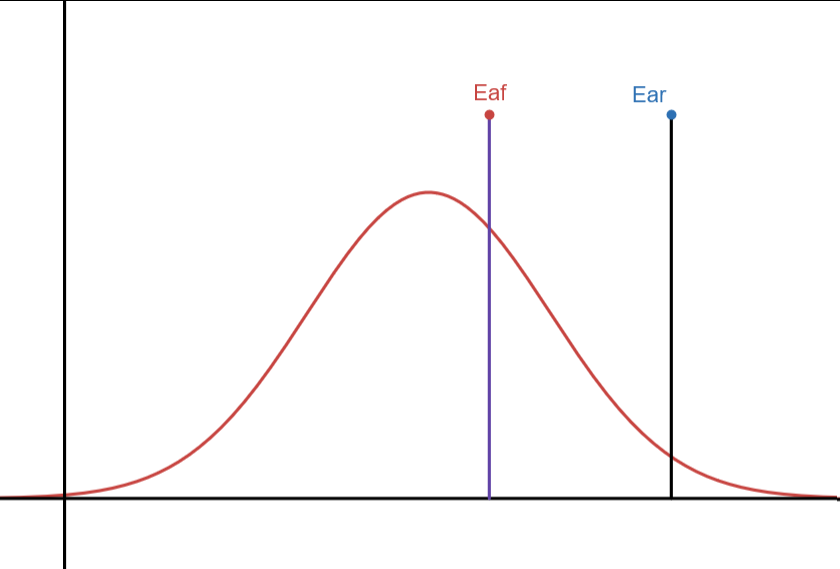
\includegraphics[width=\textwidth]{../images/tempupkei.png}
        \caption{KE graph before temperature increase}
        \label{fig:ke-pe-before}
    \end{subfigure}\hfill
    \begin{subfigure}{0.48\textwidth}
        \centering

        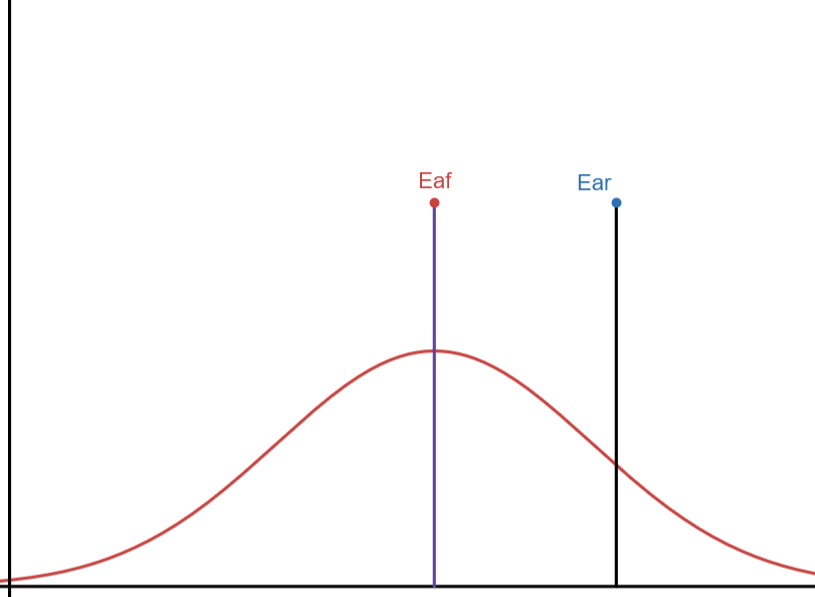
\includegraphics[width=\textwidth]{../images/tempupkef.png}
        \caption{KE graph after temperature increase}
        \label{fig:ke-pe-after}
    \end{subfigure}
    \caption{KE graphs before and after temperature change.}
\end{figure}

\begin{figure}[H]
    \centering
    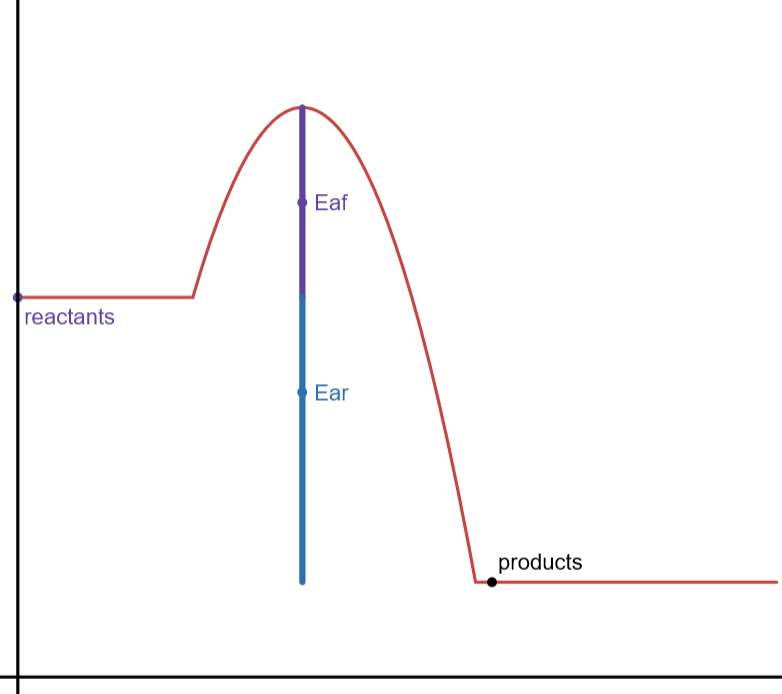
\includegraphics[width=0.48\textwidth]{../images/nochangepe.png}
    \caption{PE graph before and after temperature change.}
    \label{fig:pe-no-change}
\end{figure}

At equilibrium, the forward and reverse rates of the system were equal. However, the PE graph shows that the exothermic forward reaction requires a much lower $E_a$ than the endothermic reverse reaction. This manifests in the KE graph as a much lower percentage of particles being over the $E_{a(r)}$ compared to particles being over the $E_{a(f)}$. When the temperature was increased, the KE curve flattened and shifted to the right. While both reaction rates increased, the reverse reaction rate increased by a much greater multiple compared to the forward reaction rate. (Roughly 4x vs. 2x by inspecting the conceptual graphs).

This imbalance in reaction rates of $R_f < R_r$ resulted in the equilibrium shifting left, as more brown reactants were produced to restore balance.
~
\\
~
\\

When the temperature is decreased, the opposite happens, where the area under the KE curve over $E_{a(r)}$ decreases by a much greater multiple than the area under the KE curve over $E_{a(f)}$. With $R_f > R_r$, the system produced more colourless products and shifted right.
~
\\
~
\\
This analysis is consistent with the observed colour changes and Le Chatelier's principle, confirming that the reaction is exothermic with the enthalpy term on the right.
